\documentclass[11pt,a4paper]{ivoa} 
\input tthdefs
\input gitmeta
\usepackage{todonotes}

\usepackage{listings}
\lstloadlanguages{XML,sh,SQL}
\lstset{flexiblecolumns=true,tagstyle=\ttfamily, showstringspaces=False}

\usepackage{multirow}

\title{Simple Cone Search}

\ivoagroup{Data Access Layer}

\author[http://www.ivoa.net/twiki/bin/view/IVOA/RayPlante]{Raymond Plante}
\author[http://www.ivoa.net/twiki/bin/view/IVOA/MarcoMolinaro]{Marco Molinaro}
%\author[http://www.ivoa.net/twiki/bin/view/IVOA/MarkusDemleitner]{Markus Demleitner}
\author[http://www.ivoa.net/twiki/bin/view/IVOA/BobHanisch]{Robert Hanisch}
\author[http://www.ivoa.net/twiki/bin/view/IVOA/AlexSzalay]{Alex Szalay}
\author[http://www.ivoa.net/twiki/bin/view/IVOA/RoyWilliams]{Roy Williams}

\editor{Ray Plante, Marco Molinaro}

\previousversion[http://www.ivoa.net/Documents/ConeSearch/20200828/index.html]{WD 1.1 2020-08-28}
\previousversion[http://www.ivoa.net/Documents/REC/DAL/ConeSearch-20080222.html]{REC 1.03}
\previousversion[http://www.ivoa.net/Documents/PR/DAL/ConeSearch-20070914.html]{PR 1.02 2007-09-14}
\previousversion[http://www.ivoa.net/Documents/PR/DAL/ConeSearch-20070628.html]{PR 1.01 2007-06-28}
\previousversion[http://www.ivoa.net/Documents/PR/DAL/ConeSearch-20060908.html]{PR 1.00 2006-09-08}
       

\begin{document}

\begin{abstract} This specification defines a simple
query protocol for retrieving records from a catalog of astronomical
sources. The query describes sky position and an angular distance,
defining a cone on the sky. The response returns a list of astronomical
sources from the catalog whose positions lie within the cone, formatted
as a VOTable. This version of the specification is essentially a
transcription of the original Cone Search specification in order to move
it into the IVOA standardization process. \end{abstract}


\section*{Acknowledgments} 

This document was originally published as a
document of the US National Virtual Observatory (NVO)\footnote{The NVO
document: "Conesearch definition" (Roy Williams, Bob Hanish, Alex
Szalay; April 2002) is currently available at this link:
\url{https://wiki.ivoa.net/internal/IVOA/ConeSearch/NVO\_conesearch\_April2002.html.}}
and then transcribed into an IVOA standards document format to become
an IVOA Recommendation. The changes made in this transcription and in
the process of producing the first recommendation are reported in
Appendix \ref{appendix:nvochanges}.

The Simple Cone Search version 1.03 document has been developed with
support from the National Science Foundation's Information Technology
Research Program under Cooperative Agreement AST0122449 with The Johns
Hopkins University.

The ConeSearch-1.1 revision has been initially supported under the
ASTERICS and ESCAPE projects (funded by the European Commission
Framework Programme Horizon 2020 Research and Innovation Action, grant
agreements n. 653477 and n. 824064 respectively). Work done within the
two projects has been reported in \ref{appendix:first11changes}.

\section{Introduction}

This specification describes how a provider of an astronomical source
catalog can publish that catalog to the Virtual Observatory in such a
way that a simple cone search can be done. The data remains in the
control of the data provider, served through a web server to the world,
but the query profile and response profile are carefully controlled, as
described below. It is intended that setting up this web service be
simple enough that data providers will not have to spend too much time
on it (their funding to support such services is typically small). At
the same time, the service implementation and the data it provides can
serve as a basis for more sophisticated tools.

This specification does not specify how Cone Search services are
implemented, or how the data are stored or manipulated. The concern of
this specification is how the data are exposed to the world through
well-defined requests and responses.

This specification assumes that the data provider has already selected a
catalog of astronomical sources. This catalog can be presented as a
single table; it is expected that the table contains several columns.

\subsection{Role within the VO Architecture}

\begin{figure} \centering
%% Get the architecture diagram from the TCG chair %
%http://wiki.ivoa.net/twiki/bin/view/IVOA/IvoaTCG % If they give you a
%PDF, for now dumb it down to a png by % convert -antialias -density
%72x72 archdiag.pdf archdiag.png % Oh -- Notes don't need this; you'd
%have to remove archdiag.png % from FIGURES in the Makefile, too.
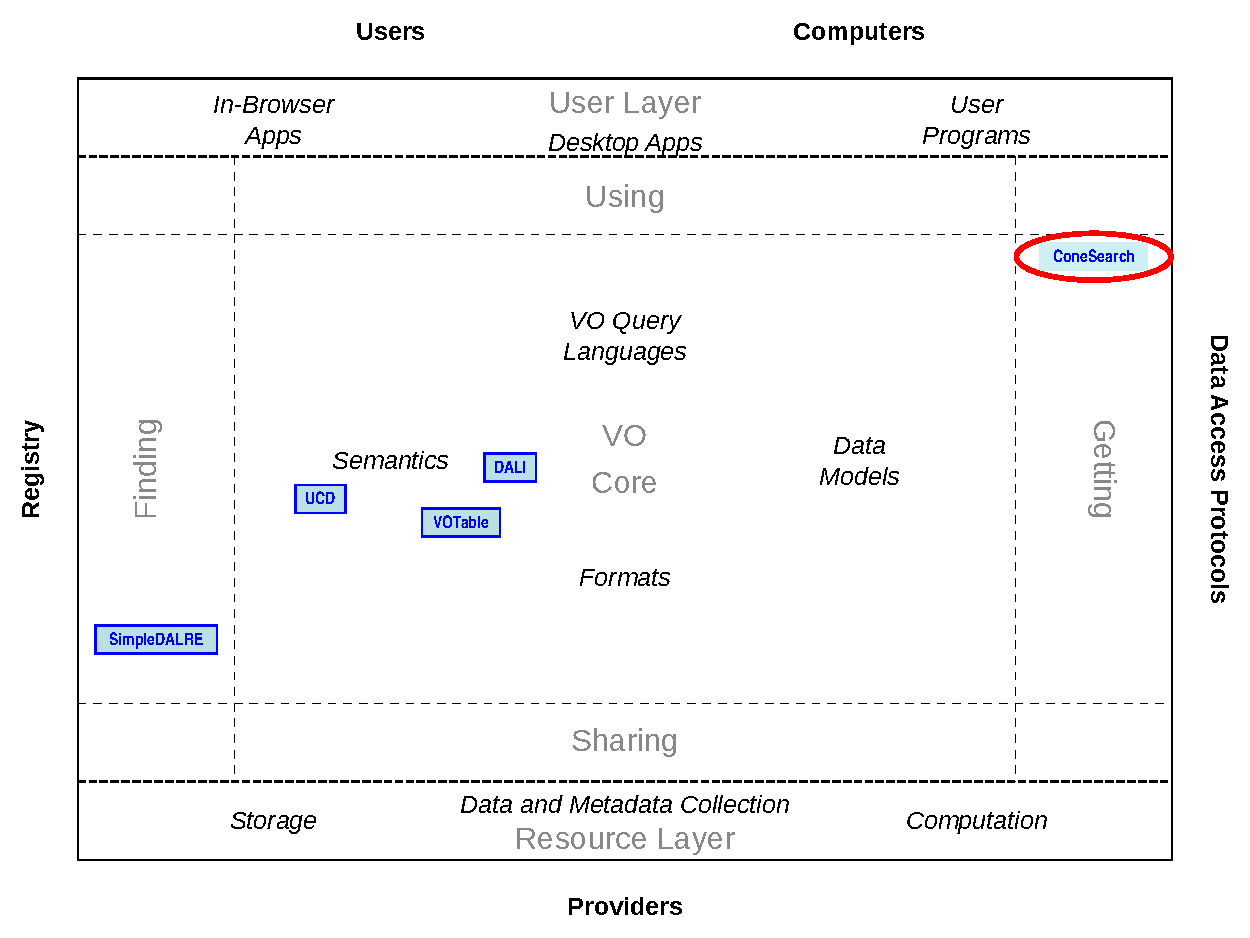
\includegraphics[width=0.9\textwidth]{role_diagram}
\caption{Architecture diagram for the Simple Cone Search
specification.}
\label{fig:archdiag} 
\end{figure}

Fig.~\ref{fig:archdiag} shows the role this document plays within the
IVOA architecture \citep{2024ivoa.spec.1114E}.

ConeSearch-1.1 makes use of the following standards:

\begin{bigdescription}
\item[DALI] \citet{2017ivoa.spec.0517D} gives the basic rules all modern
DAL protocols have to follow. This revision of the ConeSearch is meant to
align as much as possible with it.

\item[VOTable] \citet{2025ivoa.spec.0116O} defines the mandatory response
format for ConeSearch services. 

\item[UCD] \citet{2005ivoa.spec.0819D} gives a lightweight semantic
annotation that allows clients to identify the main elements in the
ConeSearch results.

\item[SimpleDALRegExt] \citet{2022ivoa.spec.0222D} currently contains
the metadata schema used to register ConeSearch version 1 services.

\end{bigdescription}

\section{Service Interface Requirements}
\label{sec:2}

A service implementation that is compliant with this standard must meet
the requirements described in the following 3 subsections
(\ref{subsec:baseurl}, \ref{subsec:response}, and \ref{subsec:error}).

\subsection{Query resource}
\label{subsec:baseurl}

The service must respond to a HTTP (or HTTPS) GET request
represented by a URL having two parts:\\ 

	\begin{itemize}
		\item A base URL of the form\\
		
		\url{http[s]://<server-address>/<path>?[<extra-GET-arg>&[...]]}\\
		
			where <server-address> and <path> are URI-compliant components
			indicating the domain address and local location path where the service
			is deployed. The <server-address> may end with one or more locally
			supported URL arguments, <extra-GET-arg>; these arguments are not
			recognized parts of the Cone Search protocol and thus are treated
			opaquely by clients of the service as part of the base URL.\\ Note that
			when it contains extra GET arguments, the base URL ends in an ampersand,
			\&; if there are no extra arguments, then it ends in a question mark,
			?.\\ 
		
		\begin{bigdescription}
			\item[Examples]
				\url{https://mycone.org/cgi-bin/VOsearch?}\\
				\url{http://adil.ncsa.uiuc.edu/vocone?resolv&issurvey=T&}
		\end{bigdescription} 
		
		Every query to a given cone search service uses the same base URL.
		
		\item Constraints expressed as a list of
			ampersand-delimited GET arguments of the form: <name>=<value> where
			<name> is a parameter name specified by this specification and <value>
			is its value. The constraints represent the query parameters which can
			vary for each successive query. The order of the name-parameter pairs is
			not significant.
		\item The baseURL and constraint list are concatenated
			to form the query. 
		\item The set of query constraints MUST include the
			following parameters, which are interpreted by the service with the
			stated meaning: 
			\begin{description}
				\item[\textbf{RA}] a right-ascension
					in the ICRS coordinate system for the positon of the center of the cone
					to search, given in decimal degrees.
				\item[\textbf{DEC}] a declination
					in the ICRS coordinate system for the positon of the center of the cone
					to search, given in decimal degrees.
				\item[\textbf{SR}] the radius of the cone to search, given in decimal degrees.
					If set to zero (SR=0) it should not return an error condition because the
					request might describe an interest in retrieving only the metadata structure
					of the service's response (i.e. discovery of the FIELDs delivered by the service).
					Returning data alongside metadata with SR=0 is also allowed.
					The metadata enquiry behaviour is similar to setting MAXREC=0, i.e. a service
					metadata request as prescribed 	by DALI\footnote{SR=0 is kept in this version 
					of this specification for back compatibility. It is suggested to prefer the
					usage of MAXREC to enable metadata discovery} \citep{2017ivoa.spec.0517D}.
			\end{description}
			\begin{bigdescription}
				\item[Example]
					\url{https://mycone.org/cgi-bin/search?RA=180.567&DEC=-30.45&SR=0.0125}
			\end{bigdescription}
		\item As defined by DALI a service SHOULD also understand the following parameters:
			\begin{description}
				\item[\textbf{MAXREC}] to let the client limit the number of records returned
					or require a service metadata response.
				\item[\textbf{RESPONSEFORMAT}] to allow alternative optional response
					formats other than the mandatory VOTable one. Indeed, a Simple
					Cone Search service MUST provide responses in VOTable format \citep{2025ivoa.spec.0116O},
					compliant with respect to what will
					be detailed in the next subsection (Sec.~\ref{subsec:response}), but should also
					support the DALI RESPONSEFORMAT parameter.
			\end{description}
		\item The query MAY contain the optional parameter,
			\textbf{VERB}, whose value is an integer--either 1, 2, or 3--indicating
			verbosity which determines how many columns are to be returned in the
			resulting table. Support for this parameter by a Cone Search service
			implementation is optional. If the service supports the parameter, then
			when the value is 1, the response should include the bare minimum of
			columns that the provider considers useful in describing the returned
			objects (while still remaining compliant with this standard; see section
			\ref{subsec:response} below). When the value is 3, the service should return all of the
			columns that are available for describing the objects. A value of 2 is
			intended for requesting a medium number of columns between the minimum
			and maximum (inclusive) that are considered by the provider to most
			typically useful to the user. When the VERB parameter is not provided,
			the server should respond as if VERB=2. If the VERB parameter is not
			supported by the service, the service should ignore the parameter and
			should always return the same columns for every request.
		\item There may be other parameters in the query, but this document does not
			specify their meaning or usage. If a query includes an optional parameter,
			either one specified by this document or not, that is not supported by
			the service implementation, the service can ignore it. In this
			case it is encouraged to add, in the response, an INFO element with the
			\verb|name| attribute set to \verb|warning| to include the parsing report
			for the ignored parameter, like:
			\begin{lstlisting}[language=XML]
<INFO name="warning" 
      value="Unrecognized optional/custom parameters.
      Ignored: TIME, MAG_V"/>
			\end{lstlisting}
	\end{itemize}
	
	A query following this syntax represents a request for
	information on sources located within the specified cone on the sky.

\subsection{Succesful response}
\label{subsec:response}

A successful response from a Cone Search service \textbf{must} be a
table containing the astronomical sources whose positions are within the
cone described by the query parameter values described in
Sec.~\ref{subsec:baseurl}. The service implementor may decide on the exact
search criterion used to select the sources, including also other
sources outside the cone.
The response table \textbf{must} contain, alongside all possible columns
available in the served source catalog:
\begin{itemize}
	\item one string column representing an identifier for that record of the table;
	\item one numerical column representing the main value for the
		right-ascension of the source in the ICRS coordinate system;
	\item one numerical column representing the main value for the
		declination of the source in the ICRS coordinate system.
\end{itemize}
Right-ascension and declination of the output columns \textbf{MUST} be in decimal degrees.

By default, the service \textbf{must} respond with an XML document in the
VOTable\citep{2025ivoa.spec.0116O} format. However, if RESPONSEFORMAT is
set (see Sec.~\ref{subsec:baseurl}) the response table \textbf{should}
match the requested format; if this format is unsupported the request
\textbf{should} fail.

When the response is in the default VOTable format (see Appendix \ref{appendix:a}
for an example), the MIME-type of the HTTP response \textbf{should} be
set to \texttt{application/x-votable+xml}. The form
\texttt{text/xml} can optionally be used, while the
form \texttt{text/xml;votable} shall be considered legal
only for backward compatibility reasons
\footnote{
	The original NVO specification allowed a MIME-type of text/xml;votable,
	this is why for backward compatibility this is still allowed but discouraged.
}
and is strongly discouraged as it is not compliant with the MIME-type
standard \citep{std:MIME}. 

Simple Cone Search services \textbf{MUST} return VOTable
version 1 documents.

The response in VOTable format \textbf{MUST} follow the prescriptions on
VOTable usage in result contained (currently) in Sec. 4.4 of the DALI 1.1
specification. Moreover it \textbf{MUST} comply with these conditions:

\begin{itemize}
	\item There must be a single RESOURCE with \texttt{type=''results''} in the VOTable,
		and that RESOURCE must contain a single TABLE. Additional RESOURCE(s) are
		allowed to enable, e.g., DataLink service descriptors.
	\item The TABLE must have FIELDs where
		the following UCD values have been set. There must only be one FIELD
		with each of these UCDs:

	\begin{itemize}
		\item Exactly one FIELD must have ucd="meta.id;meta.main",
	 		with an array character type (fixed or variable
			length), representing an ID string for that record of the table. This
			identifier could be used to retrieve that same record again from 
			that same table; the identifier string may be repeated;
		\item Exactly one FIELD must have ucd="pos.eq.ra;meta.main",
			representing the right-ascension of the source in the ICRS coordinate system.
		\item Exactly one FIELD must have ucd="pos.eq.dec;meta.main",
			representing the declination of the source in the ICRS coordinate system.
		\item The above right-ascension and declination FIELD(s) must have the datatype
			attribute set to float or double, following the VOTable
			standard \citep{2025ivoa.spec.0116O}.
	\end{itemize}

	\item The VOTable may include an expression of the
		uncertainty of the positions given in the above mentioned fields to be
		interpreted either as a positional error of the source positions, or an
		angular size if the sources are resolved. If this uncertainty is not
		provided, it should be taken to be zero; otherwise, it may be set for
		all table entries with a PARAM in the RESOURCE which has a UCD that is
		set to phys.angSize;obs and has a value which is the angle in decimal
		degrees. Alternatively, a different value for each row in the table can
		be given via a FIELD in the table having a UCD set to phys.angSize;obs.
	\item There may be other FIELDs in the table. Their specification should
		include a description, data-type, and UCD.
\end{itemize}
	
\subsection{Error response}
\label{subsec:error}

If the service detects an exceptional condition, it \textbf{should} return
an error document with an appropriate status code, as specified by DALI,
with, possibly, a Content-Type header to tell the client the format of
the document.

In the case the error is expressed in VOTable format, recommendation
expressed in Section 4.4 of DALI \textbf{should} be followed.

Errors \textbf{must} be reported in any of the following cases:
\begin{itemize}
	\item any of the three required paramaters (RA, DEC, SR) is missing;
	\item	their values cannot be parsed to floating point numbers;
	\item the value numbers are out of range (DEC=91.0, for example).
\end{itemize}

The service may also return an error if the search radius (given by the
SR parameter) is larger than the one set by the maxSR element of the
capability of the service described as a VO resource (see
Sec.~\ref{sec:3}).

Queries targeting no records \textbf{should not} generate an error
response but an empty metadata one (if applicable by format).

\section{The Resource Profile}
\label{sec:3} 

To describe a Cone Search service as a VOResource record the service
provider \textbf{must} follow the 
SimpleDALRegExt \citep{2022ivoa.spec.0222D} Recommendation (version 1.2
at the time of writing).
More in detail, Section 2 (common requirements for Simple DAL Services)
and Section 3.1 (for the specific extension definition for
Simple Cone Search) must be followed.

ConeSearch services, described as above, should be discoverable by means
of queries to a Registry RegTAP \citep{2024ivoa.spec.1002D} interface, like:
\begin{lstlisting}[language=SQL]
SELECT ivoid, res_title, access_url, std_version
FROM rr.resource
  NATURAL JOIN rr.capability
  NATURAL JOIN rr.interface 
WHERE
  standard_id LIKE 'ivo://ivoa.net/std/conesearch%'
  AND intf_role='std'
\end{lstlisting}

The \texttt{std\_version} attribute (i.e the version of the interface's
capability) could help, if present on the registered resource, to inform
the client application about the ConeSearch version the service is
following.

\appendix

\section{Sample VOTable Response}
\label{appendix:a}

This is a sample of a legal response to a Cone Search query, freely modified
from an actual query to the SIMBAD Simple Cone Search interface.

\begin{lstlisting}[language=XML,basicstyle=\footnotesize]
<?xml version="1.0" encoding="utf-8"?>
<VOTABLE version="1.4" 
  xmlns="http://www.ivoa.net/xml/VOTable/v1.3" 
  xmlns:xsi="http://www.w3.org/2001/XMLSchema-instance" 
  xsi:schemaLocation="http://www.ivoa.net/xml/VOTable/v1.3 
          http://www.ivoa.net/xml/VOTable/votable-1.4.xsd">
  <RESOURCE name="simbad_cone-search_result" type="results">
    <INFO name="standardID" 
      value="ivo://ivoa.net/std/conesearch">IVOID of the service specification</INFO>
    <INFO name="data_ivoid" 
      value="ivo://cds.simbad">IVOID of underlying data collection</INFO>
    <INFO name="publisher"
      value="CDS/SIMBAD">Data centre that produced the VOTable</INFO>
    <INFO name="article" 
      value="10.1051/aas:2000332">Bibcode or DOI of a reference article</INFO>
    <INFO name="server_software" 
      value="SIMBAD-ConeSearch/2.7-SNAPSHOT (Strasbourg)">Software version</INFO>
    <INFO name="service_protocol" value="ivo://ivoa.net/std/conesearch">
      IVOID of the protocol through which the data was retrieved</INFO>
    <INFO name="request" 
      value="https://simbad.cds.unistra.fr/cone/
             ?RA=10.684709&amp;DEC=41.26875&amp;SR=0.01666&amp;VERB=1&amp;MAXREC=2000">
      Request URL including a query string</INFO>
    <INFO name="request_date" 
      value="2026-06-09T06:09:04.156417Z">Query execution date</INFO>
    <INFO name="contact" 
      value="cds-question@unistra.fr">Email or URL to contact publisher</INFO>
    <INFO name="QUERY_STATUS" value="OK">Successful query</INFO>
    <COOSYS ID="SIMBAD-COOSYS" system="ICRS" epoch="J2000" equinox="2000"/>
    <TABLE>
      <FIELD name="distance"
        datatype="float" ucd="pos.angDistance" unit="deg">
        <DESCRIPTION>
	  Distance (in degrees) between this object and the cone-search's target.
	</DESCRIPTION>
      </FIELD>
      <FIELD ID="main_id" name="main_id" 
        arraysize="*" datatype="char" ucd="meta.id;meta.main">
        <DESCRIPTION>Main identifier for an object</DESCRIPTION>
      </FIELD>
      <FIELD name="ra"
        datatype="double" ref="SIMBAD-COOSYS" ucd="pos.eq.ra;meta.main" unit="deg">
        <DESCRIPTION>Right ascension</DESCRIPTION>
      </FIELD>
      <FIELD name="dec" 
        datatype="double" ref="SIMBAD-COOSYS" ucd="pos.eq.dec;meta.main" unit="deg">
        <DESCRIPTION>Declination</DESCRIPTION>
      </FIELD>
      <FIELD arraysize="*" datatype="char" name="otype"/>
      <FIELD datatype="int" name="biblist"/>
      <DATA>
        <TABLEDATA>
          <TR>
            <TD>7.879335328886527E-7</TD>
            <TD>M  31</TD>
            <TD>10.6847083</TD>
            <TD>41.2687500</TD>
            <TD>AGN</TD>
            <TD>13679</TD>
          </TR>
          ...
        </TABLEDATA>
      </DATA>
    </TABLE>
  </RESOURCE>
</VOTABLE>
\end{lstlisting}

\section{Changes from Previous Versions}

\subsection*{Changes from WD-1.1-20200828}
\begin{itemize}
	\item intentionally moved "may not" into "may" for main ID repeatability
	\item replaced resource description with SimpleDALRegExt references
	\item clarified response behaviour when dealing with optional
parameters
	\item exemplified/explicited HTTPS being allowed
	\item included OVERFLOW indicator (updating MAXREC usage)
	\item updated all UCD(s) to conform to the UCD1+ specification
	\item explicitly stated that RA and Dec responses must be
		in units of decimal degrees
	\item re-instated changes done in the previous WD-1.1-20200828
	\item embedded errata 1, 2 and 3 for ConeSearch-1.03
	\item Complete revert of changes to restore clean 1.03 contents,
		in view of specific minor updates (listed here above)
\end{itemize}

\subsection*{Changes from REC-1.03}
\label{appendix:first11changes}
\begin{itemize}
	\item moving base URL to a plain http://server/path? format
	\item changed error response to comply with DALI
	\item changed resource metadata importing directly from SimpleDALRegExt
	\item relaxed RA and Dec FIELDs in response to allow float or double datatype
	\item no more exactly one RESOURCE in response, now stating exactly one of
		type="results"
	\item removed fixed version (1.0 or 1.1) for VOTable default response
	\item Added DALI MAXREC and RESPONSEFORMAT
	\item Added POST as optional HTTP query method
	\item Addition of authors/editors.
	\item Plain porting of the HTML document into ivoatex template,
		including change history, then modified it and reshaped.
\end{itemize}

\subsection*{Changes from PR-1.02}
\begin{itemize}
	\item converted to Recommendation
\end{itemize}

\subsection*{Changes from PR-1.01}
\begin{itemize}
	\item eliminated the
		choice of encoding an ERROR response in a PARAM that is a direct child
		of VOTABLE as this is not legal in the VOTable schema.
	\item Allowed the use of the INFO element for error messages.
	\item In examples, made sure PARAM elements have datatype attributes
	\item Corrected wording to be definitive that positions are given 
		in the ICRS coordinate system.
	\item Other typos.
\end{itemize}

\subsection*{Changes from PR-1.00}
\begin{itemize}
	\item Various typos.
	\item Clarified description of VERB parameter:
		\begin{itemize}
			\item Clarified what is meant by optional for client and server.
			\item Clarified the meaning of the values.
		\end{itemize}
	\item Explicitly mention the 3 legal locations for ERROR messages.
	\item Refer to string types as character arrays, as per the VOTable std.
	\item Prefers text/xml;content=x-votable over text/xml;votable.
	\item Added examples of error message, legal response in appendix.
\end{itemize}

\subsection*{Changes from the original NVO Specification Document}
\label{appendix:nvochanges}
\begin{itemize}
	\item References to the original HTML document have been replaced 
		with references to this IVOA specification.
	\item Replaced references to "curator" with "data
		provider" or similar wording.
	\item Replaced references to the NVO with
		references either to the IVOA or this specification, as appropriate.
	\item Ambiguous language like "perhaps" has been replaced with more
		definitive wording where appropriate. Use of the word "will" is replaced
		with "must" and "can" with "may", in accordance with the definitions set
		in the preface.
	\item Grammatical and spelling corrections have been made.
	\item The content is organized into sections typical of an IVOA spec.
	\item Description of the URL syntax is sharper, borrowing language
		from the SIA specification [SIA]. This includes:
		\begin{itemize}
			\item More explicitly specifying the form of the URL.
			\item Sharpening the definition of the input parameters.
			\item Indicating that parameter order is not significant.
			\item Stating explicitly that unsupported optional arguments
				should be ignored.
			\item Adding examples.
			\item Re-ordering information for improved flow.
		\end{itemize}
	\item The version of VOTable supported is explicitly stated.
	\item Whereas the NVO	version describes the parameter with
		ucd="OBS\_ANG-SIZE" as "an
		expression of the opening angle of the cones", this version describes it
		specifically as "an expression of the uncertainty of the positions".
	\item A note has been added to recognize the ambiguity in the location
		of the ERROR parameter.
	\item The general description of the resource
		profile has been altered to allow rendering of the metadata to change
		according to the standards and conventions of the IVOA.
	\item An	editor's note has been added that makes reference to the RM document [RM].
	\item A requirement that \textbf{MaxSR} be given in decimal
		degrees has been added. \item For the \textbf{BaseURL} resource profile
		metadatum, the example has been replaced with a reference to the BaseURL
		syntax description.
	\item An appendix has been added to describe the
		current practice for registering Cone Search services.
\end{itemize}

\bibliography{ivoatex/ivoabib,ivoatex/docrepo,ConeSearch}


\end{document}
